\documentclass[12pt,]{article}
\usepackage[left=1in,top=1in,right=1in,bottom=1in]{geometry}
\newcommand*{\authorfont}{\fontfamily{phv}\selectfont}
\usepackage[]{charter}


\usepackage[T1]{fontenc}
\usepackage[utf8]{inputenc}
\usepackage{caption}

\usepackage{abstract}
\renewcommand{\abstractname}{}    % clear the title
\renewcommand{\absnamepos}{empty} % originally center

\renewenvironment{abstract}
 {{%
    \setlength{\leftmargin}{0mm}
    \setlength{\rightmargin}{\leftmargin}%
  }%
  \relax}
 {\endlist}





\setcounter{secnumdepth}{0}


\usepackage{graphicx,grffile}
\makeatletter
\def\maxwidth{\ifdim\Gin@nat@width>\linewidth\linewidth\else\Gin@nat@width\fi}
\def\maxheight{\ifdim\Gin@nat@height>\textheight\textheight\else\Gin@nat@height\fi}
\makeatother
% Scale images if necessary, so that they will not overflow the page
% margins by default, and it is still possible to overwrite the defaults
% using explicit options in \includegraphics[width, height, ...]{}
\setkeys{Gin}{width=\maxwidth,height=\maxheight,keepaspectratio}

\title{Paper Title : Subtitle \thanks{Acknowledgements here. \textbf{Current version}: May 13, 2018;
\textbf{Corresponding author}:
\href{mailto:apoorval@stanford.edu}{\nolinkurl{apoorval@stanford.edu}}.}  }



\author{\Large Apoorva Lal\vspace{0.05in} \newline\normalsize\emph{Stanford University}  }


\date{}

\usepackage[T1]{fontenc}
\usepackage[sc]{titlesec}



\usepackage[style=authoryear]{biblatex}

\addbibresource{/home/alal/Dropbox/MyLibrary.bib}


\newtheorem{hypothesis}{Hypothesis}
\usepackage{setspace}

\makeatletter
\@ifpackageloaded{hyperref}{}{%
\ifxetex
  \PassOptionsToPackage{hyphens}{url}\usepackage[setpagesize=false, % page size defined by xetex
              unicode=false, % unicode breaks when used with xetex
              xetex]{hyperref}
\else
  \PassOptionsToPackage{hyphens}{url}\usepackage[unicode=true]{hyperref}
\fi
}

\@ifpackageloaded{color}{
    \PassOptionsToPackage{usenames,dvipsnames}{color}
}{%
    \usepackage[usenames,dvipsnames]{color}
}
\makeatother
\hypersetup{breaklinks=true,
            bookmarks=true,
            pdfauthor={Apoorva Lal (Stanford University)},
             pdfkeywords = {JEL keywords},
            pdftitle={Paper Title : Subtitle},
            colorlinks=true,
            citecolor=blue,
            urlcolor=blue,
            linkcolor=magenta,
            pdfborder={0 0 0}}
\urlstyle{same}  % don't use monospace font for urls

% set default figure placement to htbp
\makeatletter
\def\fps@figure{htbp}
\makeatother



\usepackage{amsfonts, amsmath, amssymb, amsthm, mathtools, enumitem, fancyhdr, booktabs}

  \pagestyle{fancy}
  \lhead[CO,LE]{Title (shortened if necessary)}

% fixes encodings for accented letters in bib names
\usepackage[english]{babel}

% add tightlist ----------
\providecommand{\tightlist}{%
\setlength{\itemsep}{0pt}\setlength{\parskip}{0pt}}

% math shortcuts

% command shorthand
\newcommand{\eg}{e.g., \xspace}
\newcommand{\ie}{i.e.,\xspace}
\newcommand{\etc}{etc.\@\xspace}
\newcommand{\iid}{\emph{i.i.d.}\ }
\newcommand{\etal}{et.\ al.\ }
\newcommand{\D}{\displaystyle}
\newcommand{\ba}{\begin{array}}
\newcommand{\ea}{\end{array}}
\newcommand{\be}{\begin{enumerate}}
\newcommand{\ee}{\end{enumerate}}
\newcommand{\bi}{\begin{itemize}}
\newcommand{\ei}{\end{itemize}}
\newcommand{\bs}{\begin{align}\begin{split}\nonumber}
\newcommand{\bsnumber}{\begin{align}\begin{split}}
\newcommand{\es}{\end{split}\end{align}}
\newcommand{\fns}{\singlespace\footnotesize}

% math shorthand
% nullspace
\newcommand{\nulls}{\mathrm{null}}
% range
\newcommand{\range}{\mathrm{range}}
% maximise
\newcommand{\maximise}{\operatornamewithlimits{max}}
% minimise
\newcommand{\minimise}{\operatornamewithlimits{min}}
% maximiser
\newcommand{\argmax}{\operatornamewithlimits{arg\,max}}
% minimiser
\newcommand{\argmin}{\operatornamewithlimits{arg\,min}}
% convergence in probability sideways
\def\inprobLOW{\rightarrow_p}
% convergence in probability
\def\inprobHIGH{\,{\buildrel p \over \rightarrow}\,}
% convergence in probability 2
\def\inprob{\,{\inprobHIGH}\,}
% convergence in distribution
\def\indist{\,{\buildrel d \over \rightarrow}\,}

% ellipsis
\newcommand{\tto}{,\ldots,}

% blackboard F
\def\Function{\mathbb{F}}

% Natural
\def\Nat{\mathbb{N}}
% Integers
\def\Int{\mathbb{Z}}
% Reals
\def\Real{\mathbb{R}}
% Rationals
\def\Rat{\mathbb{Q}}
% Complex
\def\Cplx{\mathbb{C}}

% n-dimensional Real
\def\Realn{\mathbb{R}^n}
% expectation_n
\def\Expn{\mathbb{E}_n}
% P_n
\def\Probn{\mathbb{P}_n}

\def\rel{\,{\buildrel R \over \sim}\,}
% generic m x n matrix
\newcommand{\gmatrix}[1]{\begin{pmatrix} {#1}_{11} & \cdots &
    {#1}_{1n} \\ \vdots & \ddots & \vdots \\ {#1}_{m1} & \cdots &
    {#1}_{mn} \end{pmatrix}}
% lagrangian
% \newcommand{\Lagr}{\mathcal{L}}
% inner product
\newcommand{\iprod}[2]{\left\langle {#1} , {#2} \right\rangle}
% vector norm
\newcommand{\norm}[1]{\left\Vert {#1} \right\Vert}
% absolute value
\newcommand{\abs}[1]{\left\vert {#1} \right\vert}
% linalg misc
\renewcommand{\det}{\mathrm{det}}
\newcommand{\rank}{\mathrm{rank}}
\newcommand{\spn}{\mathrm{span}}
\newcommand{\row}{\mathrm{Row}}
\newcommand{\col}{\mathrm{Col}}
\renewcommand{\dim}{\mathrm{dim}}
% weakly prefer
\newcommand{\prefeq}{\succeq}
% strictly prefer
\newcommand{\pref}{\succ}
% sequence
\newcommand{\seq}[1]{\{{#1}_n \}_{n=1}^\infty }
% single arrow
\renewcommand{\to}{{\rightarrow}}
% double arrow
\newcommand{\corres}{\overrightarrow{\rightarrow}}
% evaluate definite integral
\newcommand*\Eval[3]{\left.#1\right\rvert_{#2}^{#3}}
% expectation
\newcommand{\Exp}[1]{\mathbb{E}\left(#1\right)}
% variance
\newcommand{\Var}[1]{\mathbb{V}\left(#1\right)}

\makeatletter
\def\@maketitle{%
  \newpage
  \begin{center}%
  \let \footnote \thanks
    {\fontsize{24}{24}\selectfont\raggedright  \@title}
  \end{center}
}
%\fi
\makeatother


\begin{document}

% \pagenumbering{arabic}% resets `page` counter to 1
%



\maketitle

{% \usefont{T1}{pnc}{m}{n}
\thispagestyle{plain}
{ \selectfont
\maketitle  % title \par
}

\begin{center}
{
   \vskip 13.5pt\relax \normalsize\fontsize{14}{14}
\textbf{Apoorva Lal} \hskip 15pt \emph{\small Stanford University}   
}
\end{center}
}





\begin{abstract}

    \hbox{\vrule height .2pt width 39.14pc}

    \vskip 8.5pt % \small

\noindent abstract goes here


\vskip 8.5pt \noindent \emph{Keywords}: JEL keywords \par

    \hbox{\vrule height .2pt width 39.14pc}



\end{abstract}


\vskip 6.5pt

{
\hypersetup{linkcolor=black}
\setcounter{tocdepth}{3}
\tableofcontents
}

\newpage


\noindent \doublespacing \hypertarget{introduction}{%
\section{Introduction}\label{introduction}}

Main question: What is the average air speed velocity of a laden
swallow?

\textcite{Deatonanalysishouseholdsurveys1997}

The quick brown fox jumped over the lazy dog\footnote{but the dog's
  laziness is heavily debated}.

\hypertarget{model}{%
\section{Model}\label{model}}

\begin{align*}
\maximise_{c_t,k_{t+1}} &  \sum_{t=1}^{\infty} \beta^t u(c_t)  \\
  s.t. & \enspace c_{t} + k_{t+1} \leq f(k_t) + (1-\delta)k_t
\end{align*}

\hypertarget{estimation-framework}{%
\section{Estimation Framework}\label{estimation-framework}}

\begin{align*}
\text{outcome}_{ict} = \alpha_i & + \sum_{k=0}^2 \beta_{t-k}^p
PPI_{ict-k} + \gamma_{ct} + \epsilon_{ict} \\
\text{outcome}_{ict} = \alpha_i & + \sum_{k=0}^2 \beta_{t-k}^p PPI_{ict-k} +
\sum_{k=0}^2 + \beta_{t-k}^m CPI_{ict-k} + \\ & \gamma_{c}\times
trend_t + \epsilon_{ict}
\end{align*}

\hypertarget{data}{%
\section{Data}\label{data}}

\hypertarget{make-plots-in-document}{%
\subsection{Make plots in document}\label{make-plots-in-document}}

\begin{figure}
\centering
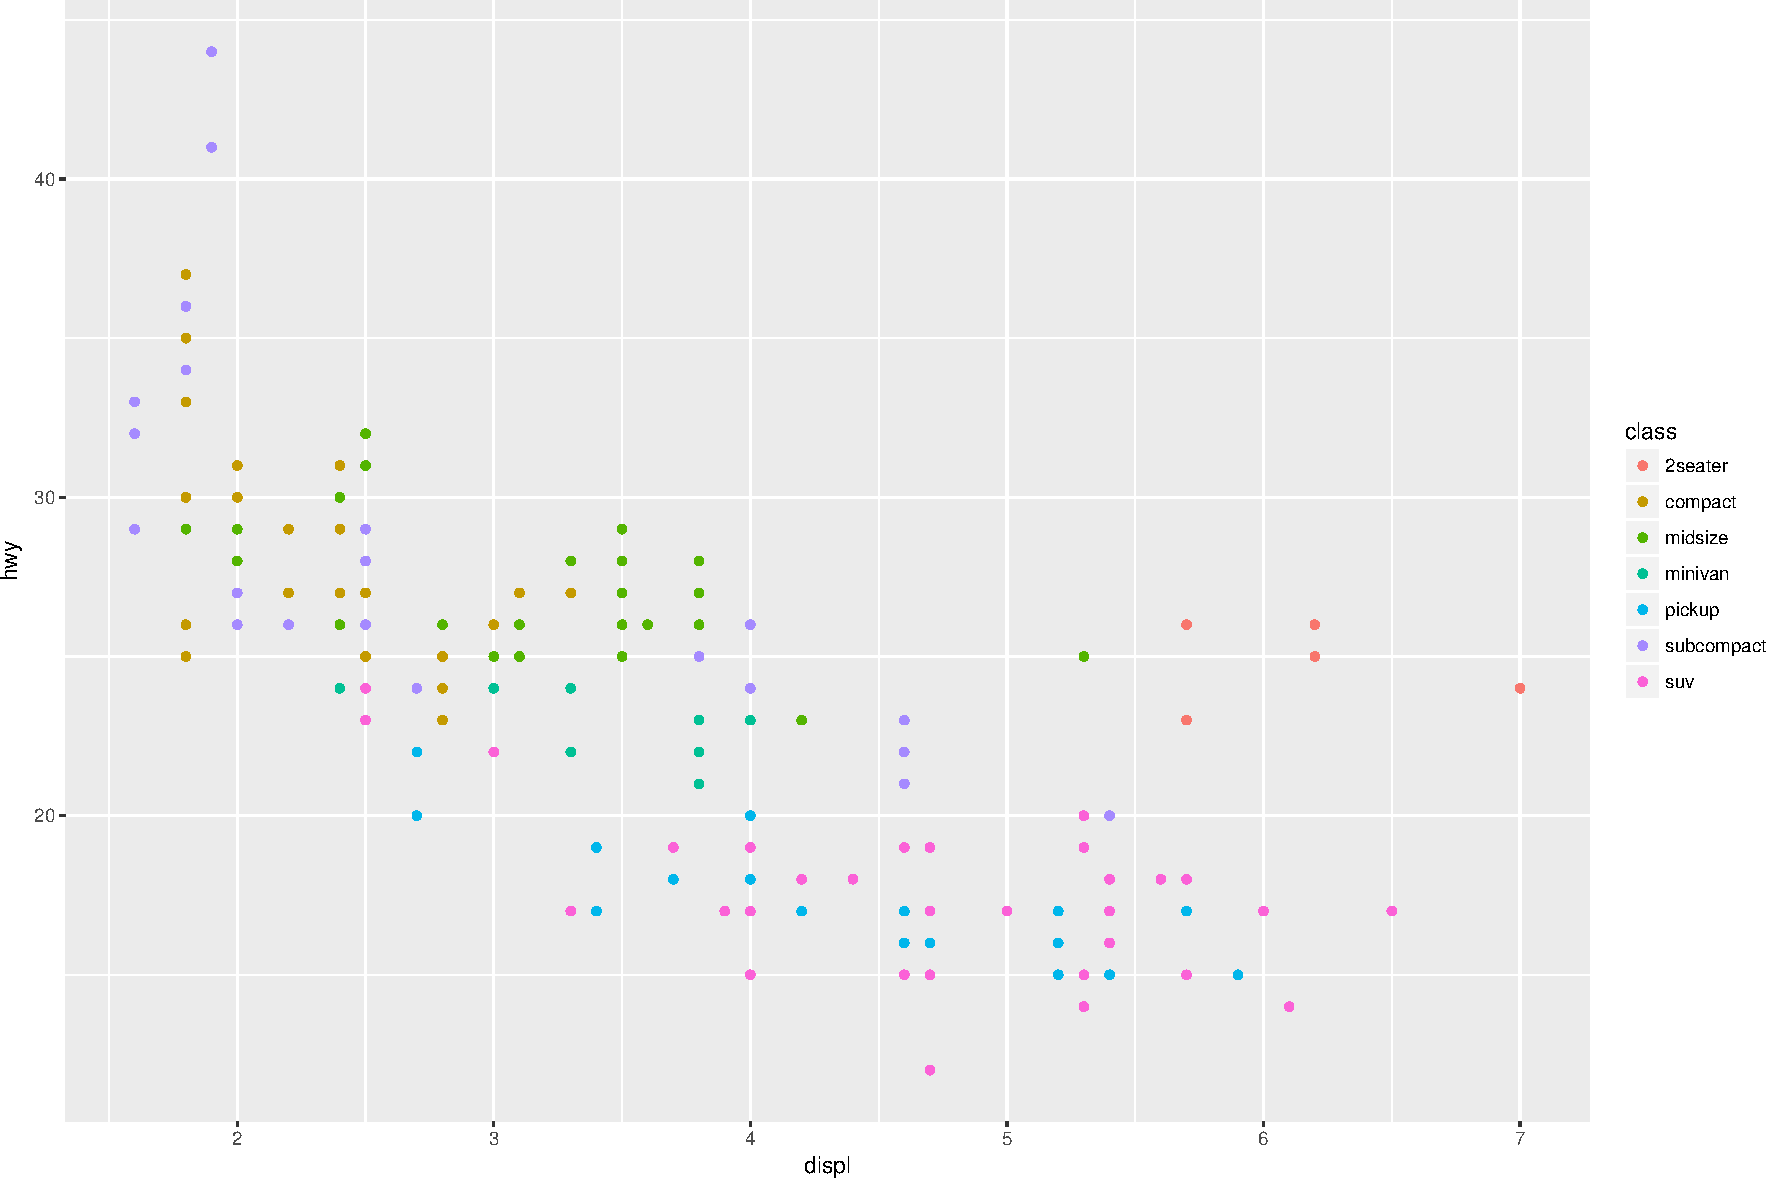
\includegraphics{Figs/unnamed-chunk-2-1.pdf}
\caption{Made here}
\end{figure}

\newpage

\hypertarget{embedded-plots}{%
\subsection{Embedded plots}\label{embedded-plots}}

\begin{figure}
\centering
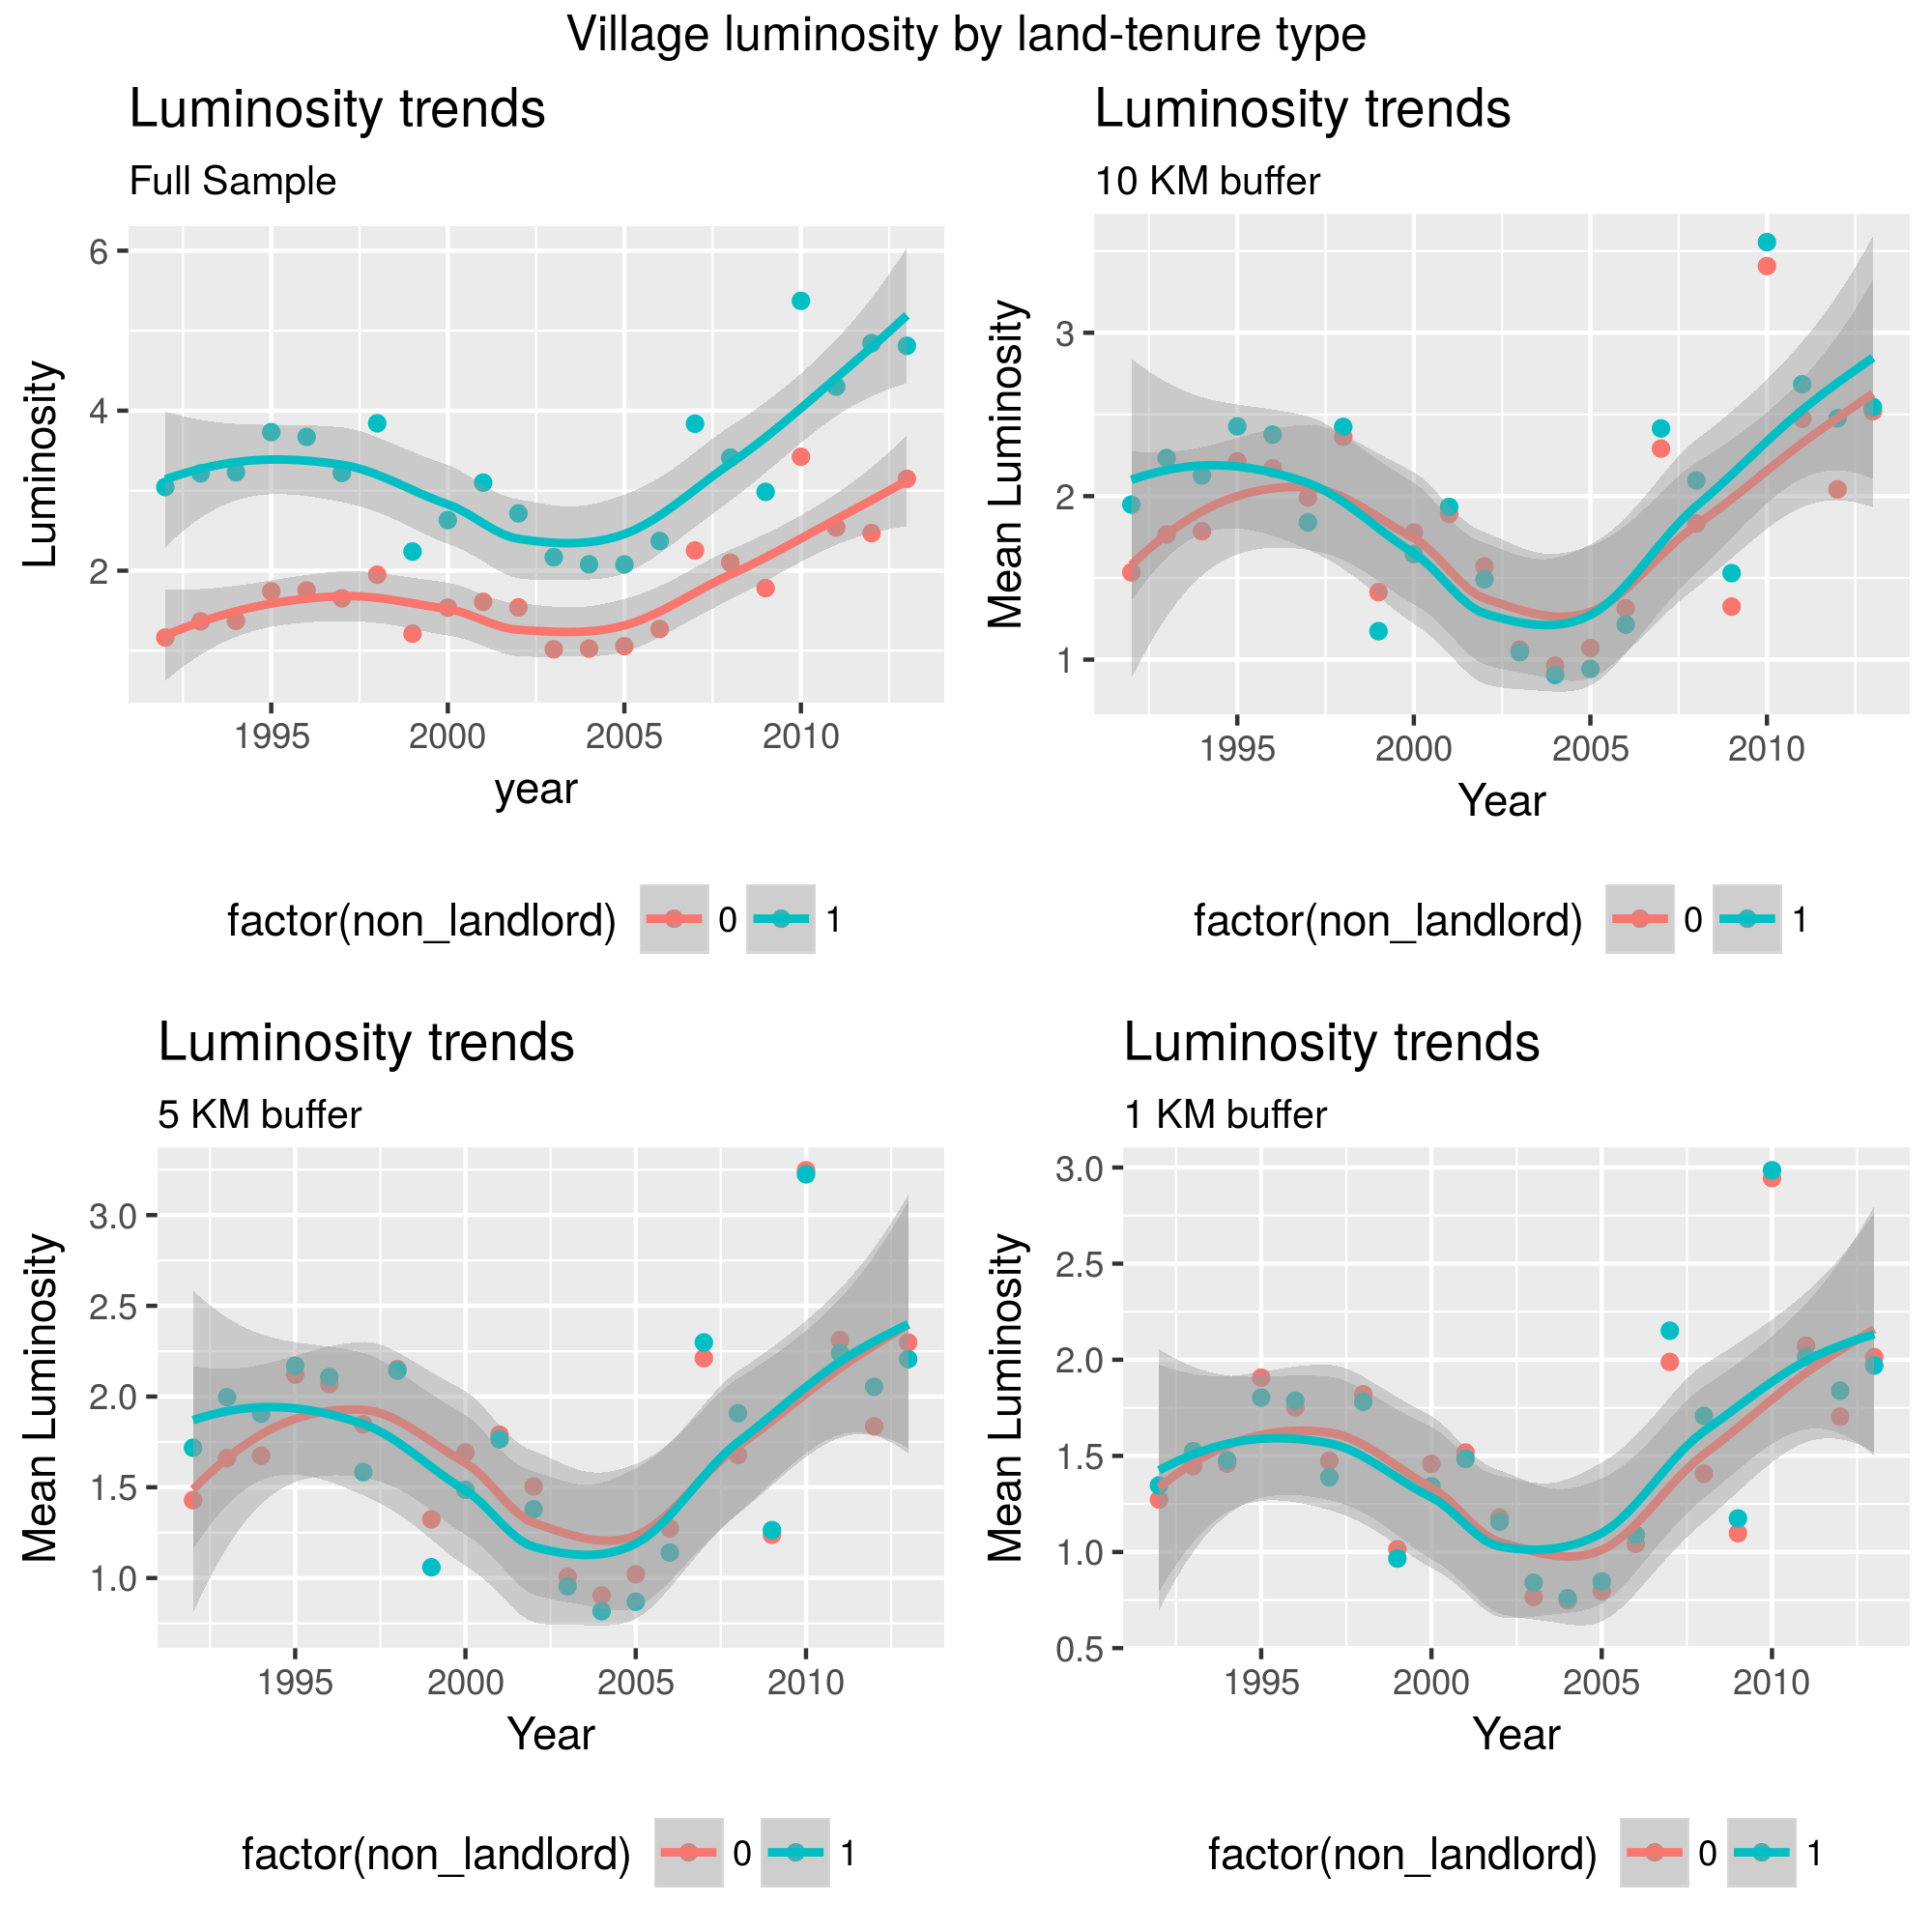
\includegraphics{Figs/luminosity_grid.png}
\caption{Made somewhere else}
\end{figure}

\newpage

\hypertarget{results}{%
\section{Results}\label{results}}

\hypertarget{embed-stargazer-output}{%
\subsection{Embed stargazer output}\label{embed-stargazer-output}}

\begin{table}[!htbp] \centering 
  \caption{} 
  \label{} 
\begin{tabular}{@{\extracolsep{5pt}}lc} 
\\[-1.8ex]\hline 
\hline \\[-1.8ex] 
 & \multicolumn{1}{c}{\textit{Dependent variable:}} \\ 
\cline{2-2} 
\\[-1.8ex] & hwy \\ 
\hline \\[-1.8ex] 
 cyl & $-$1.685$^{***}$ \\ 
  & (0.142) \\ 
  & \\ 
 factor(class)compact & $-$2.238$^{*}$ \\ 
  & (1.336) \\ 
  & \\ 
 factor(class)midsize & $-$2.027 \\ 
  & (1.311) \\ 
  & \\ 
 factor(class)minivan & $-$6.112$^{***}$ \\ 
  & (1.462) \\ 
  & \\ 
 factor(class)pickup & $-$9.555$^{***}$ \\ 
  & (1.279) \\ 
  & \\ 
 factor(class)subcompact & $-$1.663 \\ 
  & (1.335) \\ 
  & \\ 
 factor(class)suv & $-$8.410$^{***}$ \\ 
  & (1.240) \\ 
  & \\ 
 Constant & 38.280$^{***}$ \\ 
  & (1.639) \\ 
  & \\ 
\hline \\[-1.8ex] 
Observations & 234 \\ 
R$^{2}$ & 0.808 \\ 
Adjusted R$^{2}$ & 0.802 \\ 
Residual Std. Error & 2.649 (df = 226) \\ 
F Statistic & 135.900$^{***}$ (df = 7; 226) \\ 
\hline 
\hline \\[-1.8ex] 
\textit{Note:}  & \multicolumn{1}{r}{$^{*}$p$<$0.1; $^{**}$p$<$0.05; $^{***}$p$<$0.01} \\ 
\end{tabular} 
\end{table}

\hypertarget{embed-standalone-latex-table}{%
\subsection{Embed standalone latex
table}\label{embed-standalone-latex-table}}

\vspace{5mm}
{
\def\sym#1{\ifmmode^{#1}\else\(^{#1}\)\fi}
\begin{tabular}{l*{4}{c}}
\toprule
                    &\multicolumn{1}{c}{(1)}&\multicolumn{1}{c}{(2)}&\multicolumn{1}{c}{(3)}&\multicolumn{1}{c}{(4)}\\
                    &\multicolumn{1}{c}{Linear}&\multicolumn{1}{c}{Quadratic}&\multicolumn{1}{c}{Spline}&\multicolumn{1}{c}{Interaction}\\
                    &        b/se       &        b/se       &        b/se       &        b/se       \\
\midrule
Population Growth   &       0.054\sym{*}&       0.180\sym{*}&                   &       0.085\sym{*}\\
                    &    (0.0017)       &    (0.0043)       &                   &    (0.0053)       \\
Population Growth Squared&                   &      -0.053\sym{*}&                   &                   \\
                    &                   &    (0.0017)       &                   &                   \\
pop\_growth: below median&                   &                   &       0.097\sym{*}&                   \\
                    &                   &                   &    (0.0023)       &                   \\
pop\_growth: above median&                   &                   &      -0.071\sym{*}&                   \\
                    &                   &                   &    (0.0049)       &                   \\
above\_median=1 $\times$ Population Growth&                   &                   &                   &      -0.025\sym{*}\\
                    &                   &                   &                   &    (0.0042)       \\
Constant            &      -0.045\sym{*}&      -0.096\sym{*}&      -0.072\sym{*}&      -0.054\sym{*}\\
                    &    (0.0016)       &    (0.0023)       &    (0.0019)       &    (0.0023)       \\
\midrule
Observations        &     1182563       &     1182563       &     1182563       &     1182563       \\
\(R^{2}\)           &       0.001       &       0.002       &       0.002       &       0.001       \\
\bottomrule
\end{tabular}
}

\vspace{5mm}

\hypertarget{conclusion}{%
\section{Conclusion}\label{conclusion}}

Something significant

\hypertarget{appendix}{%
\section{Appendix}\label{appendix}}




\newpage
\singlespacing
\printbibliography[title=Bibliography]

\end{document}
